%Stratospheric Ballooning Assoication
%2014-2015 Brochure
%Matthew Nelson

%Document class, page setup
\documentclass[10pt,foldmark,notumble]{leaflet}
\renewcommand*\foldmarkrule{.3mm}
\renewcommand*\foldmarklength{5mm}
\makeatletter

%Declare packages to use
%\usepackage{amsmath}
\usepackage[T1]{fontenc}
\usepackage{textcomp}
\usepackage{float}
\usepackage{multicol}
\usepackage{wrapfig}
\usepackage{mathptmx}
\usepackage[scaled=0.9]{helvet}
\usepackage[hidelinks]{hyperref}
\usepackage{graphicx}
\usepackage[dvipsnames,usenames]{color}
%--------------------------------------------------------------
%Configure page
\def\ptmTeX{T\kern-.1667em\lower.5ex\hbox{E}\kern-.075emX\@}
\DeclareRobustCommand{\ptmLaTeX}{L\kern-.3em
        {\setbox0\hbox{T}%
         \vbox to\ht0{\hbox{%
         \csname S@\f@size\endcsname
         \fontsize\sf@size\z@
         \math@fontsfalse\selectfont
         A}%
         \vss}%
        }%
        \kern-.12em
        \ptmTeX}
\makeatother
\let\TeX=\ptmTeX
\let\LaTeX=\ptmLaTeX
\usepackage{shortvrb}
\MakeShortVerb{\|}

%Set Fonts
\renewcommand{\descfont}{\normalfont}
\newcommand\Lpack[1]{\textsf{#1}}
\newcommand\Lclass[1]{\textsf{#1}}
\newcommand\Lopt[1]{\texttt{#1}}
\newcommand\Lprog[1]{\textit{#1}}

\newcommand*\defaultmarker{\textsuperscript\textasteriskcentered}
\renewcommand*{\familydefault}{\sfdefault}
%Disable page numbering
\pagenumbering{gobble}

%------------------------------------------------------------
%Title and author info
\title{\bf \ \\ \ \\ \ \\ \ \\SBA}

\author{%
\Large \bf Stratospheric Ballooning Association
}
\date{\bf 2014-2015 }
%------------------------------------------------------------
%Main body
\CutLine*{1}% Dotted line without scissors
\CutLine*{6}%  Dotted line without scissors

%\AddToBackground{1}{%  Background of a small page
%  \put(0,0){\textcolor{Cerulean}{\rule{\paperwidth}{\paperheight}}}}


\AddToBackground{1}{%  Background of a small page
  \put(90,460){\includegraphics[scale=0.07]{logo3_print.jpg}}}


%\AddToBackground{6}{%  Background of a small page
  %\put(0,0){\textcolor{cardinal}{\rule{\paperwidth}{\paperheight}}}}
  
%\AddToBackground{5}{%  Background of a small page
  %\put(0,0){\textcolor{gold}{\rule{\paperwidth}{\paperheight}}}}


%\AddToBackground*{2}{% Background of a large page
%  \put(\LenToUnit{.5\paperwidth},\LenToUnit{.5\paperheight}){%
%    \makebox(0,0)[c]{%
%      \resizebox{.9\paperwidth}{!}{\rotatebox{35.26}{%
%        \textsf{\textbf{\textcolor{light-red}{SBA}}}}}}}}


\begin{document}
\maketitle
\section{Who We Are}
The SBA is here to promote high altitude ballooning through empowering its members and public on high altitude ballooning, to encourage collaboration with all those that wish to participate and to advance the science, technology, engineering, operations and policy of high altitude ballooning.

\subsection{Our Mission}
The Mission of SBA is to support those engaged in high altitude ballooning by promoting the field to others, empowering practitioners, and facilitating collaboration.

\subsection{Our Vision}
The vision of SBA is to support and be the collective voice of all who are engaged in high altitude ballooning including those participating in one or more of the following areas: 
\begin{enumerate}
\item In the personal or hobby area
\item In education (K-12 and College)
\item In research
\item In the commercial area
\end{enumerate}
We are open to all those that are interested in performing high altitude balloon flights or using high altitude balloon flights for their needs.

\subsection{Our History}
The SBA started with an idea at the first Academic High Altitude Conference of having an organization that could help promote and represent those interested in high altitude ballooning.  The idea then grew at following conferences with growing interest.  In 2013 the SBA was incorporated as a non-profit organization in the state of Iowa with it being based in Ames, IA by Matthew Nelson, Jennifer Nelson and Ethan Harstad.  That same year the SBA was awarded funding from a Taylor University National Science Foundation grant to help establish and grow the organization.  

Today the SBA is a growing organization that began accepting membership at the 5th Annual Academic High Altitude Conference held at the University of North Dakota. The SBA continues to grow both its membership base and the information and benefits it provides its members. 
\ \\ \ \\ \ \\ \ \\
%\begin{wrapfigure}{R}{0.45\textwidth}
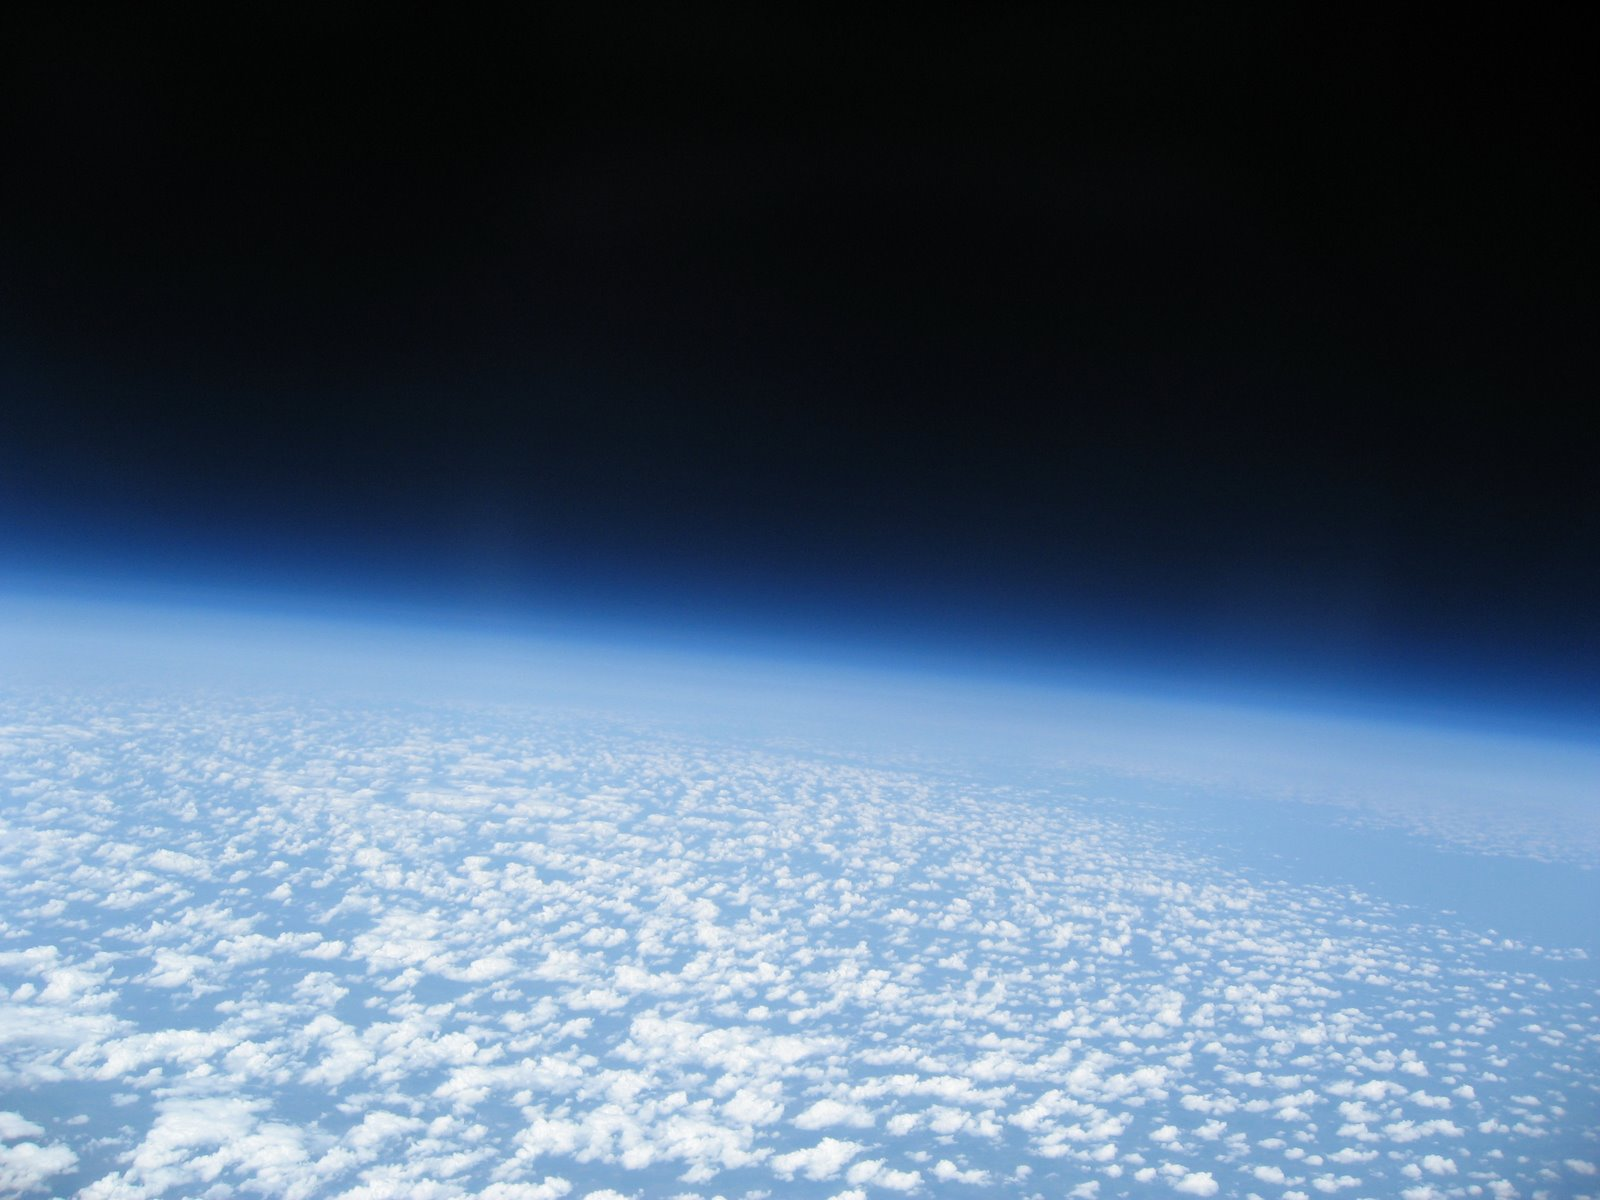
\includegraphics[scale=.2]{IMG_1921.jpg}
%\end{wrapfigure}

\section{What We Do}

The SBA is there to help their members in executing high altitude balloon launches and to do so in a safe and effective manner.  We strive to give our members the knowledge and tools that they will need to perform any kind of high altitude balloon mission.  The SBA has strong roots in academia and will continue that tradition by encouraging and providing the tools that educators can use to bring STEM education through high altitude ballooning to their classroom.

\section{Membership Benefits}
The SBA conducted a survey on what they would like to see in the SBA and the potential benefits to its members.  Based on those results, we have outlined the following membership benefits.  As the SBA grows, we expect to continue to expand and add additional benefits that will help our members to excel in high altitude ballooning.

\subsection{Academic High Altitude Conference (AHAC)}
The Academic High Altitude Conference is now in it's fifth year and is rapidly becoming the conference for not only academic interest in high altitude ballooning but for non-academic use as well.  The conference attracts presenters from academic, government and industrial leaders in high altitude ballooning.  The conference also features a two day workshop that features both a technical workshop and an educational workshop.  The conference is kicked off with an inaugural balloon launch run by the hosting entity.

%\includegraphics[scale=.09]{P6220033.jpg}

\subsection{Virtual and Mini-conference}  
Due to the popularity of AHAC, it is proposed that 2-4 hour mini-conferences occur virtually over the internet, perhaps during the fall and spring. Papers, breakout sessions, keynotes, etc. may be included.

\subsection{SBA Website}
The SBA website is your portal to information on high altitude ballooning.  These resources include access to current and past papers and presentations from the Academic High Altitude Conference, How to Videos, access to experts, access to flight prediction software, and information about current and past flights.  Additional content and information will be added in the future.

\subsection{Annual Journal}
SBA is working with the editor of the Transactions of the Canadian Society of Mechanical Engineering (a peer reviewed journal) towards a special issue on high altitude ballooning in 2015.  This will be the inaugural journal which will lay the ground work for the SBA's own journal starting in 2016. 
\ \\
\subsection{High Altitude Ballooning Best Practices}
The SBA will be facilitating a committee to work on determining areas that need best practices, creating a process for establishing best practices in these areas, and implementing this process.  This information will then be shared with members and to the public on best practices with high altitude ballooning.
\ \\
\subsection{Collaborative Grant Proposal}
The SBA is working to facilitate at least one proposal to obtain grant funding. The goal would be to submit a proposal during 2014-2015 that would be a collaboration between several SBA members. The proposal topic would be chosen based on interest of the collaborators, the available grants, and the probability of being awarded the grant.
\ \\
\section{How to Become a Member of SBA}
There are two ways to become a member.  First, your registration cost for the Academic High Altitude Conference includes membership in the SBA.  Second, starting in the Fall of 2014 we will have membership available through the SBA website.  For more information please visit our webiste.

\section{Board of Directors}
The following members currently make up the board of directors.  If you are interested in serving on the board, please contact Matthew Nelson.
\begin{center}
{\bf President} \ \\
Matthew E. Nelson\ \\
mnelson@stratoballooning.org \ \\ \ \\

{\bf 2014 - 2015 Board Members}\ \\ \ \\
\begin{multicols}{2}
Bill Brown  \ \\ Dr. Ron Fevig \ \\ Ethan Harstad \ \\ Jason Krueger \ \\ Jennifer Nelson \ \\ Dr. Don Takehara
\end{multicols}

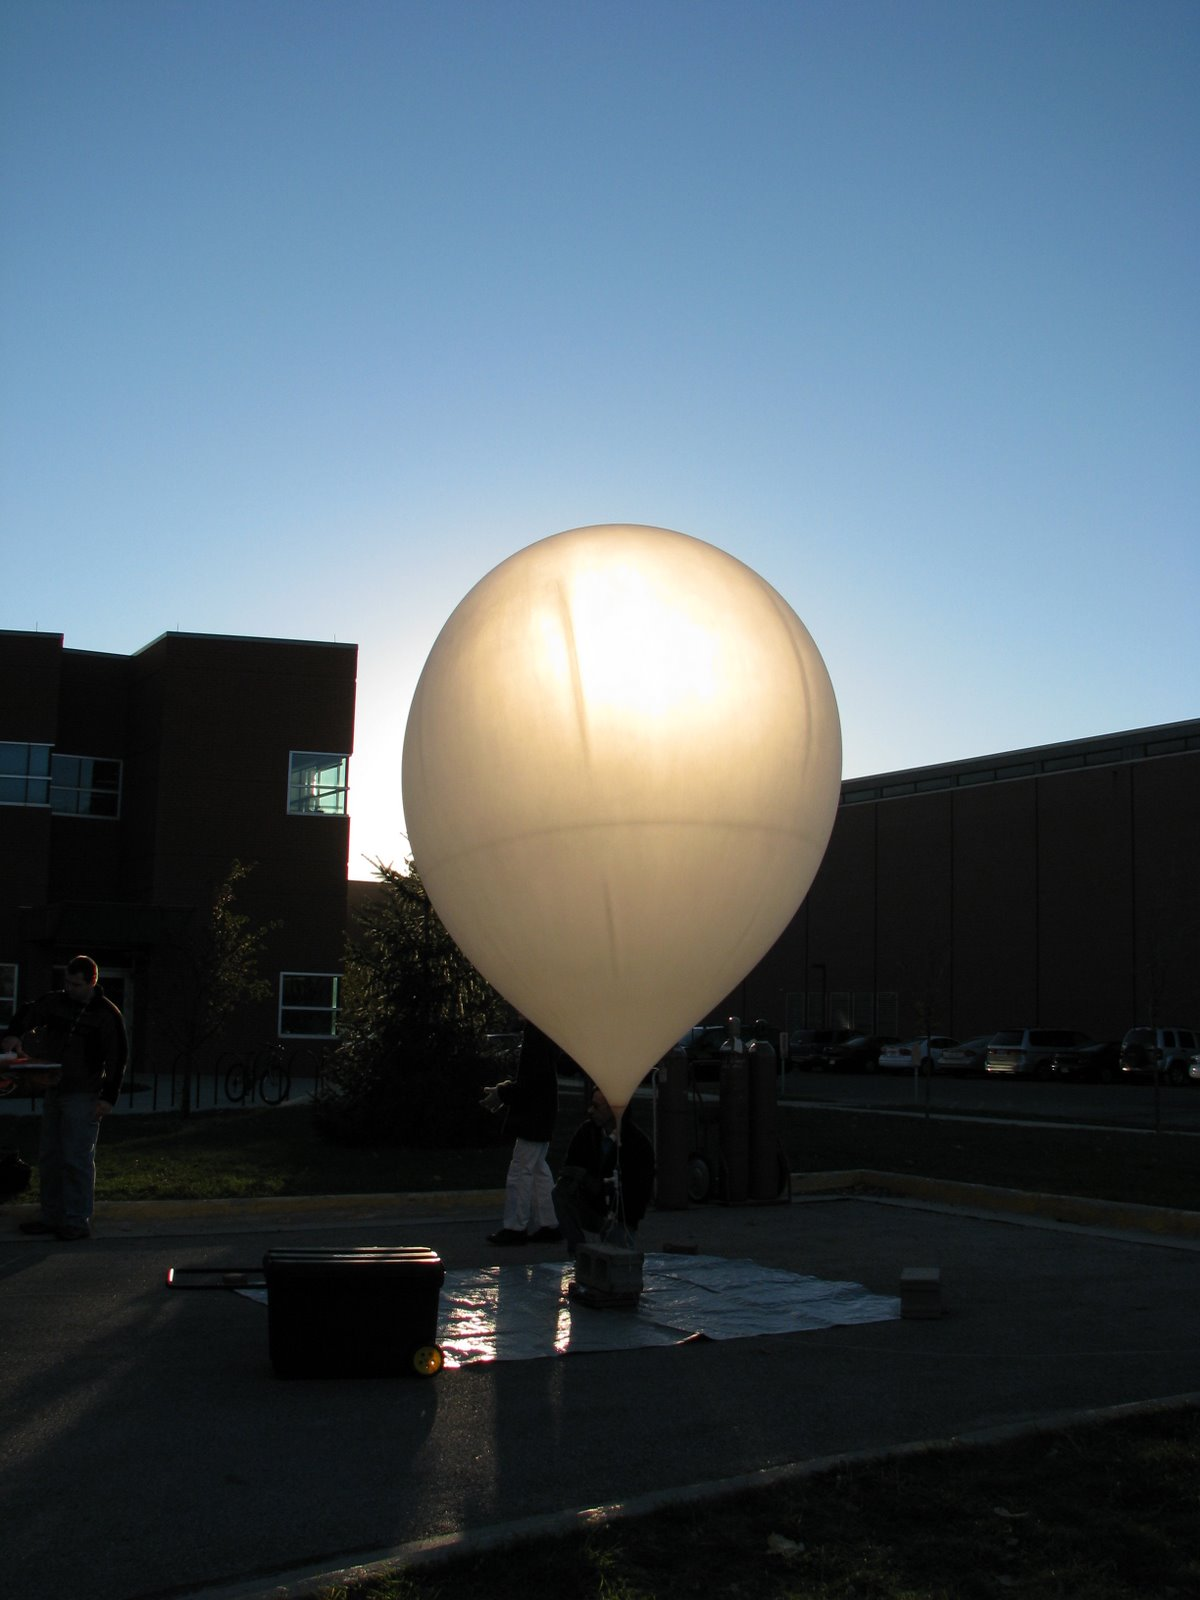
\includegraphics[scale=.23]{IMG_0826.jpg}

\end{center}
\section{Contacting the SBA}
If you wish to contact the SBA, please contact us through the following methods

\begin{center}
\vspace{0.2cm}
{\large \bf Follow us on the web: }

\bf Website\ \\ \url{http://www.stratoballooning.org}

\bf Facebook\ \\ \url{https://www.facebook.com/stratoballooning}

\bf Google+\ \\ \url{https://plus.google.com/+StratoballooningOrg}

\bf Twitter\ \\ \url{https://twitter.com/SBA_org}

\vspace{0.2cm}
{\bf Email}

info@stratoballooning.org

\vspace{0.2cm}
%{\bf Phone}

%515-555-5555

\end{center}

\end{document}